\chapter{Experiments}
In this chapter I will describe the experiments I conducted to evaluate the metrics. I will evaluate metrics of both classes: distance metric and score metric. Metrics such as FID, KID, FD\_CLIP, KD\_CLIP, FD\_DINOv2 and KD\_DINOv2 are distance metrics. While CLIPScore, ImageReward and HSPv2 are related to score metrics. All metrics will be evaluated on two datasets: COCO with 41 thousand samples and MJHQ30k with 30 thousand samples.

I will use the Imagen\cite{Imagen} diffusion model for my experiments.I will conduct the following experiments:
\begin{enumerate}
    \item Measure the quality of the model at different steps of image generation.
    \item Measure the quality of the model at different iterations of model training.
    \item Measure the quality of the model with corrupted images by overlaying black squares on the images.
\end{enumerate}
In what follows I will describe each experiment in more detail and will attach graphs and measurement results.

And it is important to note that distance metrics which used CLIP as feature extractor was measured two times: with normalized featured and without. Normalized features are marked as "CLIP\_norm", not normalized just "CLIP".
\section{Imagen}
First, I want to describe the structure of the Imagen\cite{Imagen} diffusion network. Imagen is a state-of-the-art text-to-image generation model developed by researchers at Google Research, announced in May 2022.

Imagen's diffusion model successively adds noise to an image over a series of steps until the data is completely random (pure noise). Starting from noise, the model learns to gradually denoise the data, reconstructing an image conditioned on the given text input. This is achieved through a series of learned de-noising steps.


Imagen leverages a Transformer-based \cite{Visual_transformer} architecture for conditioning on text. This allows for capturing complex relationships and semantic details from the text, integrating these into the image synthesis process more effectively than previous models like DALL-E \cite{DALLE}.

Different from some prior models, Imagen produces high-fidelity and high-resolution images by utilizing a super-resolution process. This involves generating an image at a relatively lower resolution initially and then progressively enhancing its details and resolution in subsequent stages. In summary, the essence of Imagen's diffusion model is the sophisticated use of textual description-based noise introduction and removal processes to create high-resolution photorealistic images.

In conclusion, Imagen has several distinguishing features:
\begin{enumerate}
    \item The use of a large encoder for text compared to the weight and size of the diffusion model.
    \item The use of frozen text encoder.
    \item The use of two additional diffusion models to improve image quality. These diffusion models are called "Super-Resolution Diffusion Model".
\end{enumerate}
Figure \ref{fig:Imagen_diagram} \cite{Imagen} taken from the original article shows the structure of the Imagen diffusion model.
\begin{figure}[h]
\centering
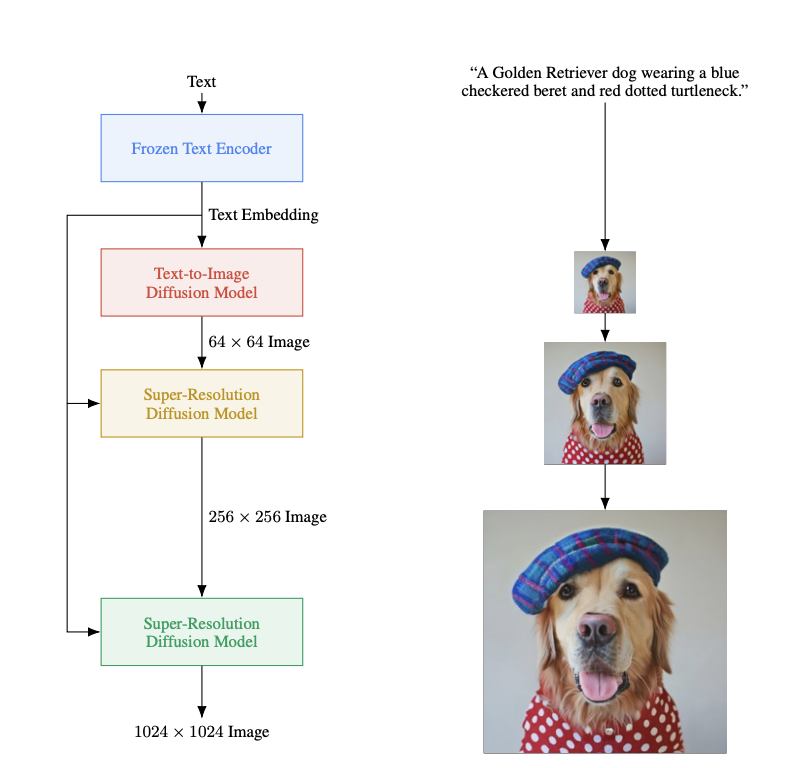
\includegraphics[width=12cm, height=12cm]{figs/Imagen_diagram.png}
\caption{Imagen diagram taken from \cite{Imagen}. Chitwan Saharia et al. highlights: "Imagen uses a frozen text encoder to encode the input text
into text embeddings. A conditional diffusion model maps the text embedding into a 64 × 64 image.
Imagen further utilizes text-conditional super-resolution diffusion models to upsample the image,
first 64 × 64 → 256 × 256, and then 256 × 256 → 1024 × 1024."\cite[p.19]{Imagen}}
\label{fig:Imagen_diagram}
\end{figure}

\section{Experiments with distance metrics}
\subsection{Different iterations of model training}
The first experiment I did was to train Imagen with different numbers of training steps, i.e. some models were undertrained. The intuition is that the image obviously gets better and better with more training steps. I purposely made a small number of steps so that the model would not have time to overtrain. I got several models: Imagen trained at 100K, 150K, 200K and 300K training steps.

I took the COCO dataset and measured the metrics on it. I plotted all distance metrics at Figure \ref{fig:coco_train_steps}. The metric correlates more strongly with human judgment if the red and blue graphs match.
The results I got from the graphs:
\begin{itemize}
    \item FID and KID correlate with human judgement well enough if metrics are calculated on COCO dataset.
    \item KD\_CLIP, FD\_CLIP, KD\_CLIP\_norm, FD\_CLIP\_norm acting weird, so there's no pattern.
    \item FD\_CLIP and FD\_CLIP\_norm are similar. KD\_CLIP and KD\_CLIP/norm are also similar
    \item FD\_DINOv2 correlates with human opinion better than any other metric.
    \item KD\_DINOv2 is completely different from a person's opinion.
\end{itemize}

I took the MJHQ30K dataset and measured the metrics on it. I plotted all distance metrics at Figure \ref{fig:mjhq30k_train_steps}. The metric correlates more strongly with human judgment if the red and blue graphs match.
The results I got from the graphs:
\begin{itemize}
    \item FID and KID correlate with human judgement well enough if metrics are calculated on MJHQ30K dataset.
    \item KD\_CLIP, FD\_CLIP, KD\_CLIP\_norm, FD\_CLIP\_norm acting weird, so there's no pattern.
    \item FD\_CLIP and FD\_CLIP\_norm are similar. KD\_CLIP and KD\_CLIP/norm are also similar
    \item FD\_DINOv2 and KD\_DINOv2 correlates with human opinion better than any other metric.
\end{itemize}

\begin{figure}[]
\centering
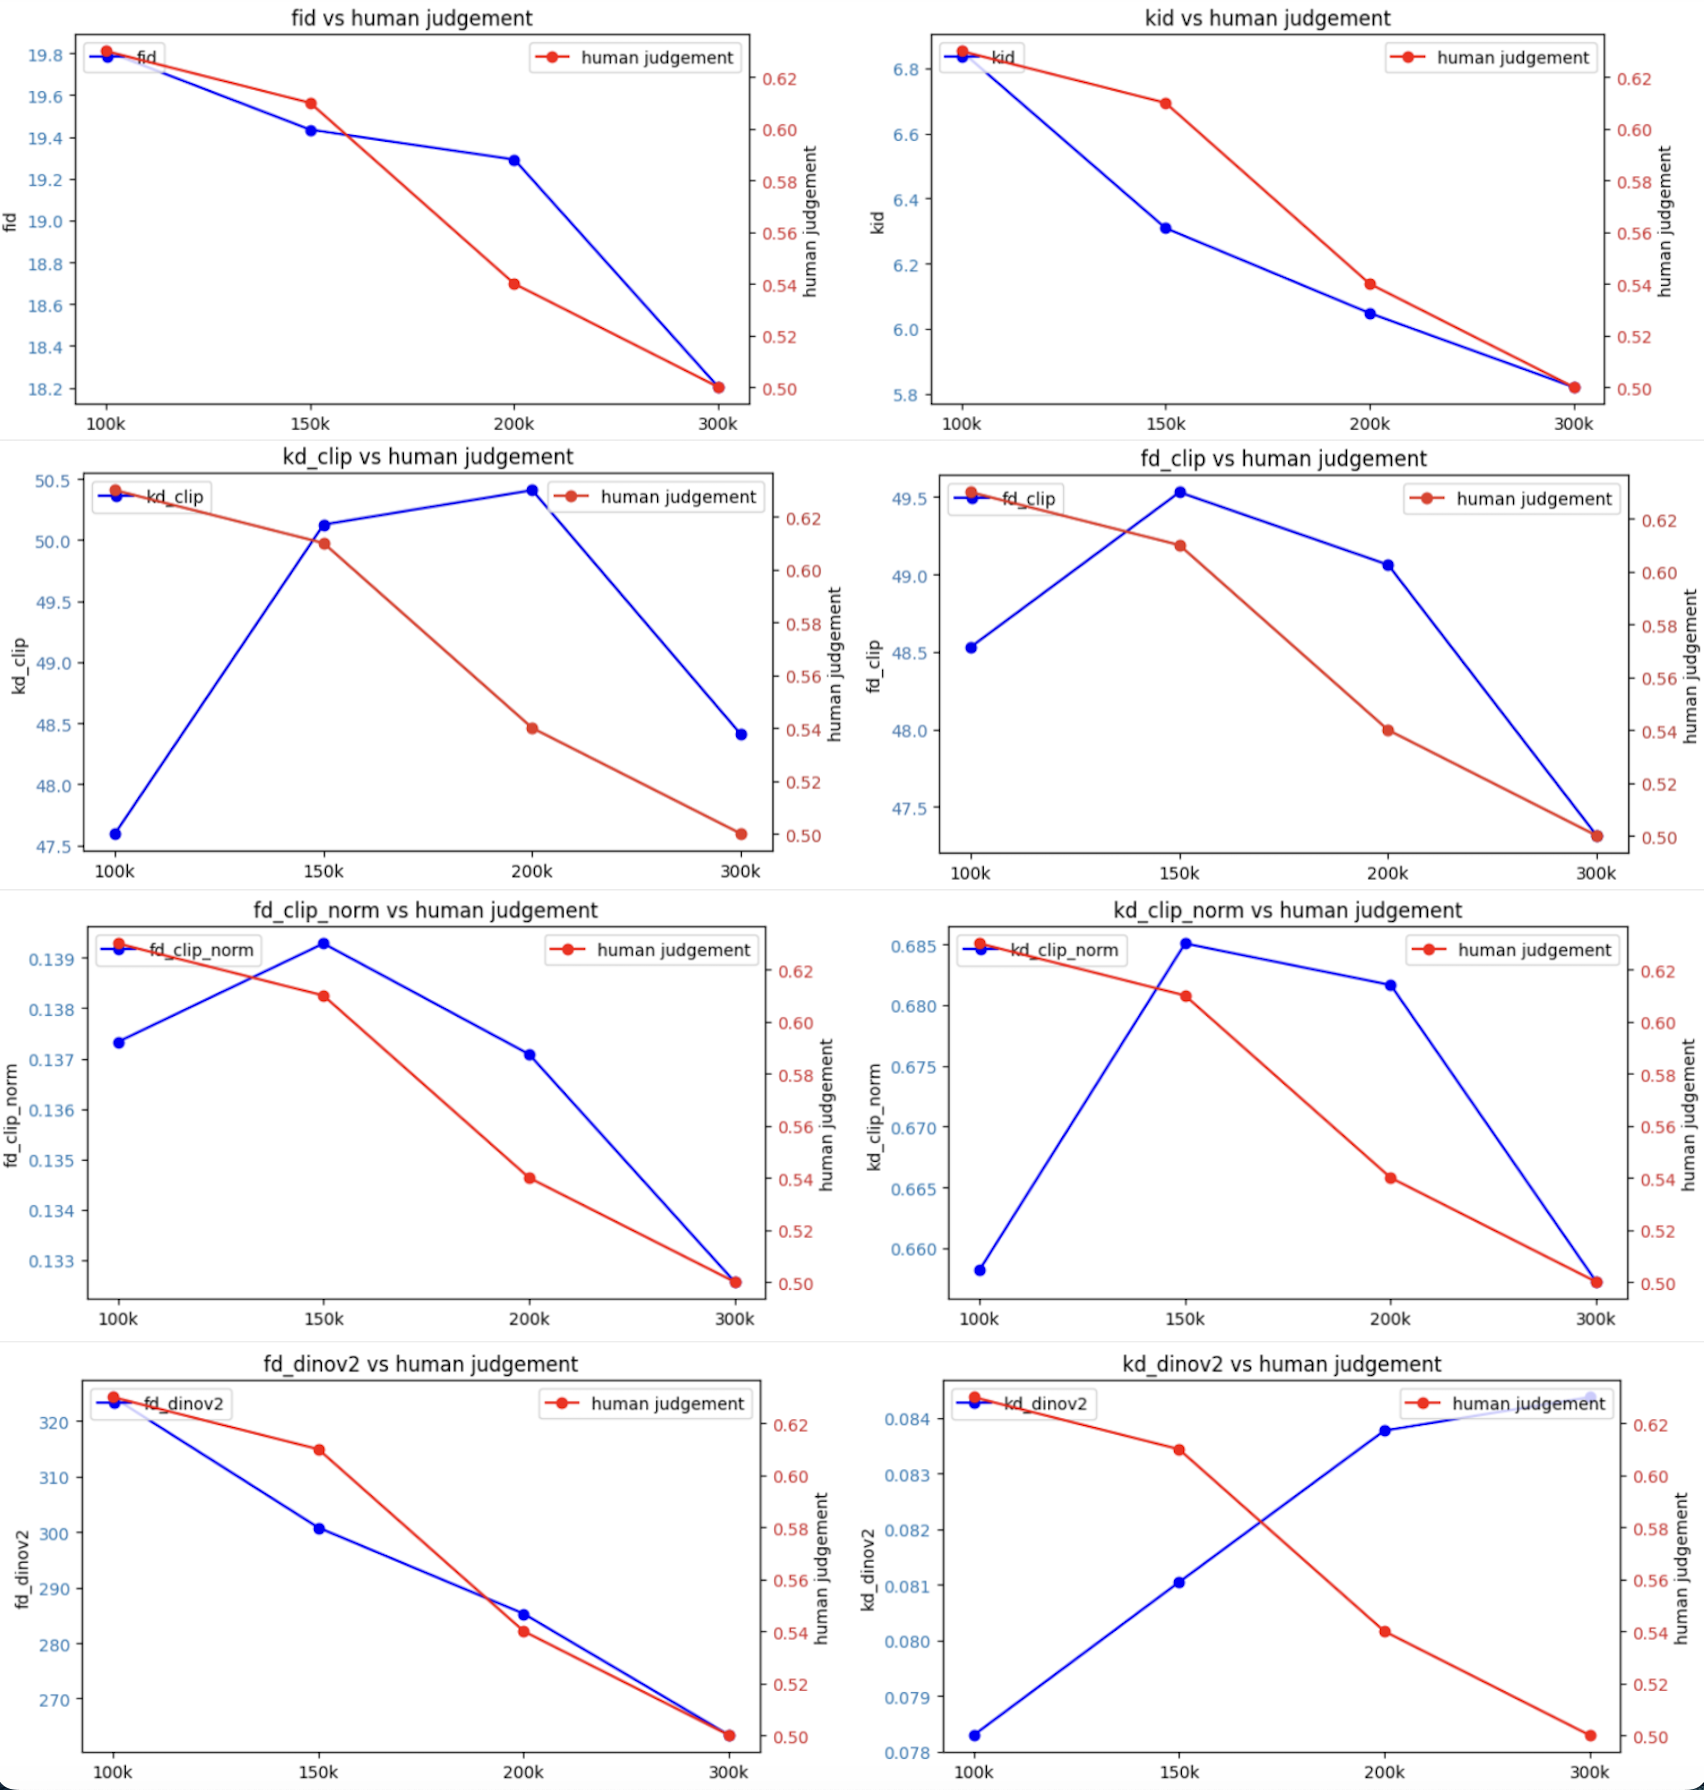
\includegraphics[width=16cm, height=17cm]{figs/coco_train_steps.png}
\caption{Distance metrics measured on COCO dataset on models with different number of train steps. On the X-axis from left to right there are models with different number of steps from smaller to larger, i.e. from 100 thousand to 300 thousand. The left Y-axis shows the results of the metric, so the blue graph corresponds to the left Y-axis. On the right Y-axis are the results of human evaluation - this is the proportion of victories of the fully trained model (i.e. the model with 300 training steps) against the current model with the current number of training steps. The red graph corresponds to the right Y-axis.}
\label{fig:coco_train_steps}
\end{figure}

\begin{figure}[]
\centering
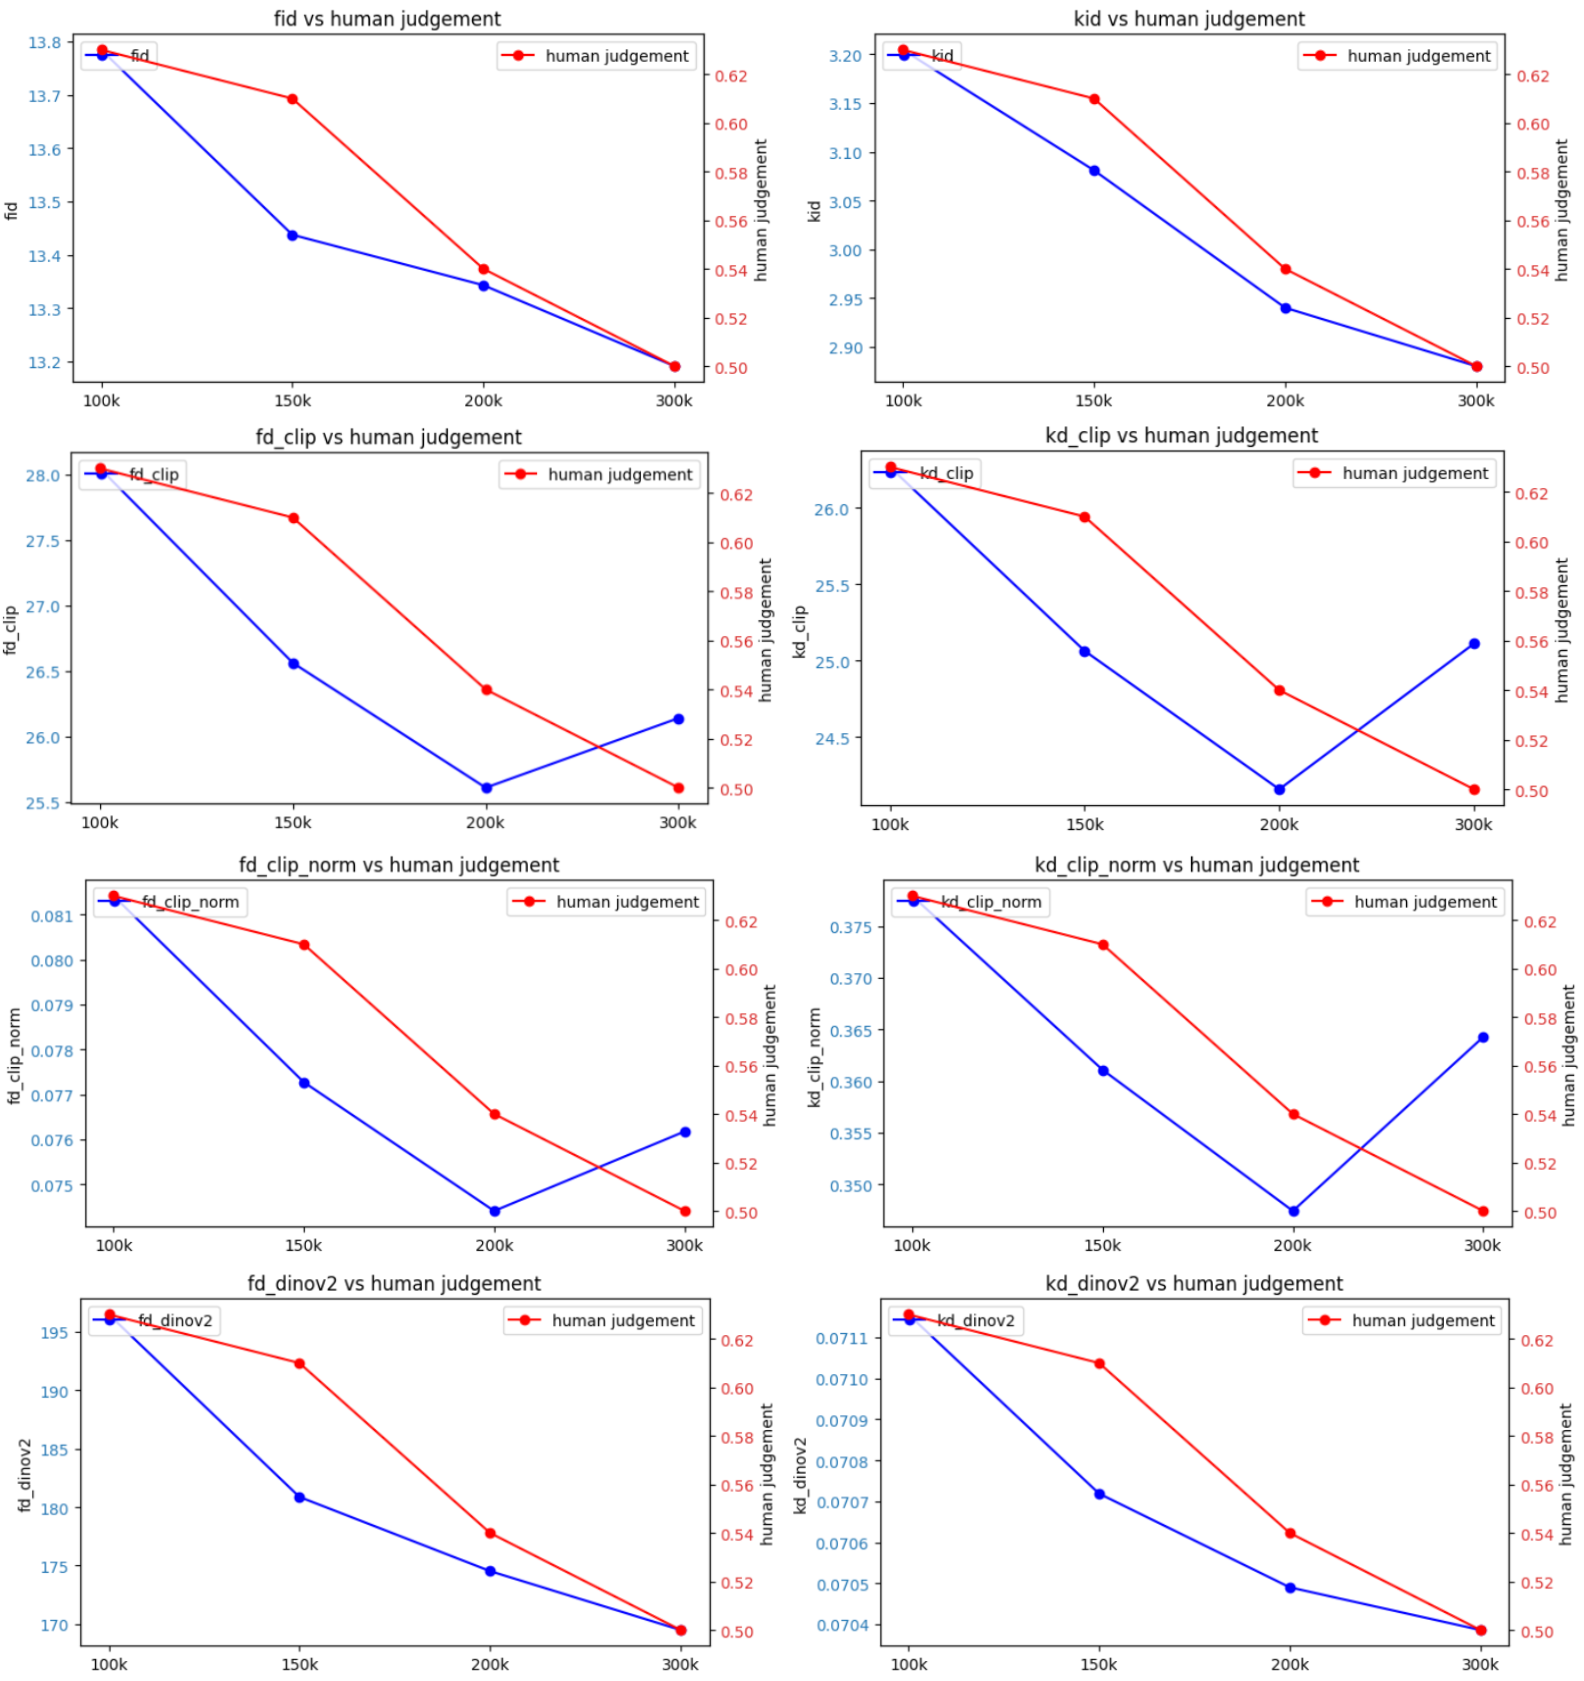
\includegraphics[width=16cm, height=17cm]{figs/mjhq30k_train_steps.png}
\caption{Distance metrics measured on MJHQ30K dataset on models with different number of train steps. The axes are the same on the Figure\ref{fig:coco_train_steps}.}
\label{fig:mjhq30k_train_steps}
\end{figure}

\subsubsection{Summary}
At the end of this experiment I can say that the FD\_DINOv2 metric performed the best. FID and KID also showed excellent results. FD\_CLIP, KD\_CLIP, FD\_CLIP\_norm and KD\_CLIP\_norm show poor results which may doubt CLIP as feature extractor. KD\_DINOv2 showed excellent results on the MJHQ30k dataset, but the exact opposite on COCO.

I have an assumption that this behavior may be due to the fact that the model generates images more similar to the images that MJHQ30K generates, i.e. contrast and aesthetics, than to the real images that are in the COCO dataset.

\subsection{Different steps of image generation}
The second experiment I did was to take the trained Imagen model and generate an image, but at different generation steps, i.e. at different de-noising steps. The intuition is that the image obviously gets better and better with more de-noising steps.

I took the COCO dataset and measured the metrics on it. I plotted all distance metrics at Figure \ref{fig:coco_gen_steps}. The metric correlates more strongly with human judgment if the red and blue graphs match.
The results I got from the graphs:
\begin{itemize}
    \item FID correlate with human judgement well enough if metrics are calculated on COCO dataset.
    \item KID, KD\_CLIP, FD\_CLIP, KD\_CLIP\_norm, FD\_CLIP\_norm acting weird, so there's no pattern.
    \item FD\_CLIP and FD\_CLIP\_norm are similar. KD\_CLIP and KD\_CLIP/norm are also similar
    \item FD\_DINOv2 correlates with human opinion better than any other metric.
    \item KD\_DINOv2 is completely different from a person's opinion, as the last experiment.
\end{itemize}

I took the MJHQ30K dataset and measured the metrics on it. I plotted all distance metrics at Figure \ref{fig:mjhq30k_gen_steps}. The metric correlates more strongly with human judgment if the red and blue graphs match.
The results I got from the graphs:
\begin{itemize}
    \item All metrics correlate with human judgement well enough if metrics are calculated on MJHQ30K dataset.
\end{itemize}

\begin{figure}[]
\centering
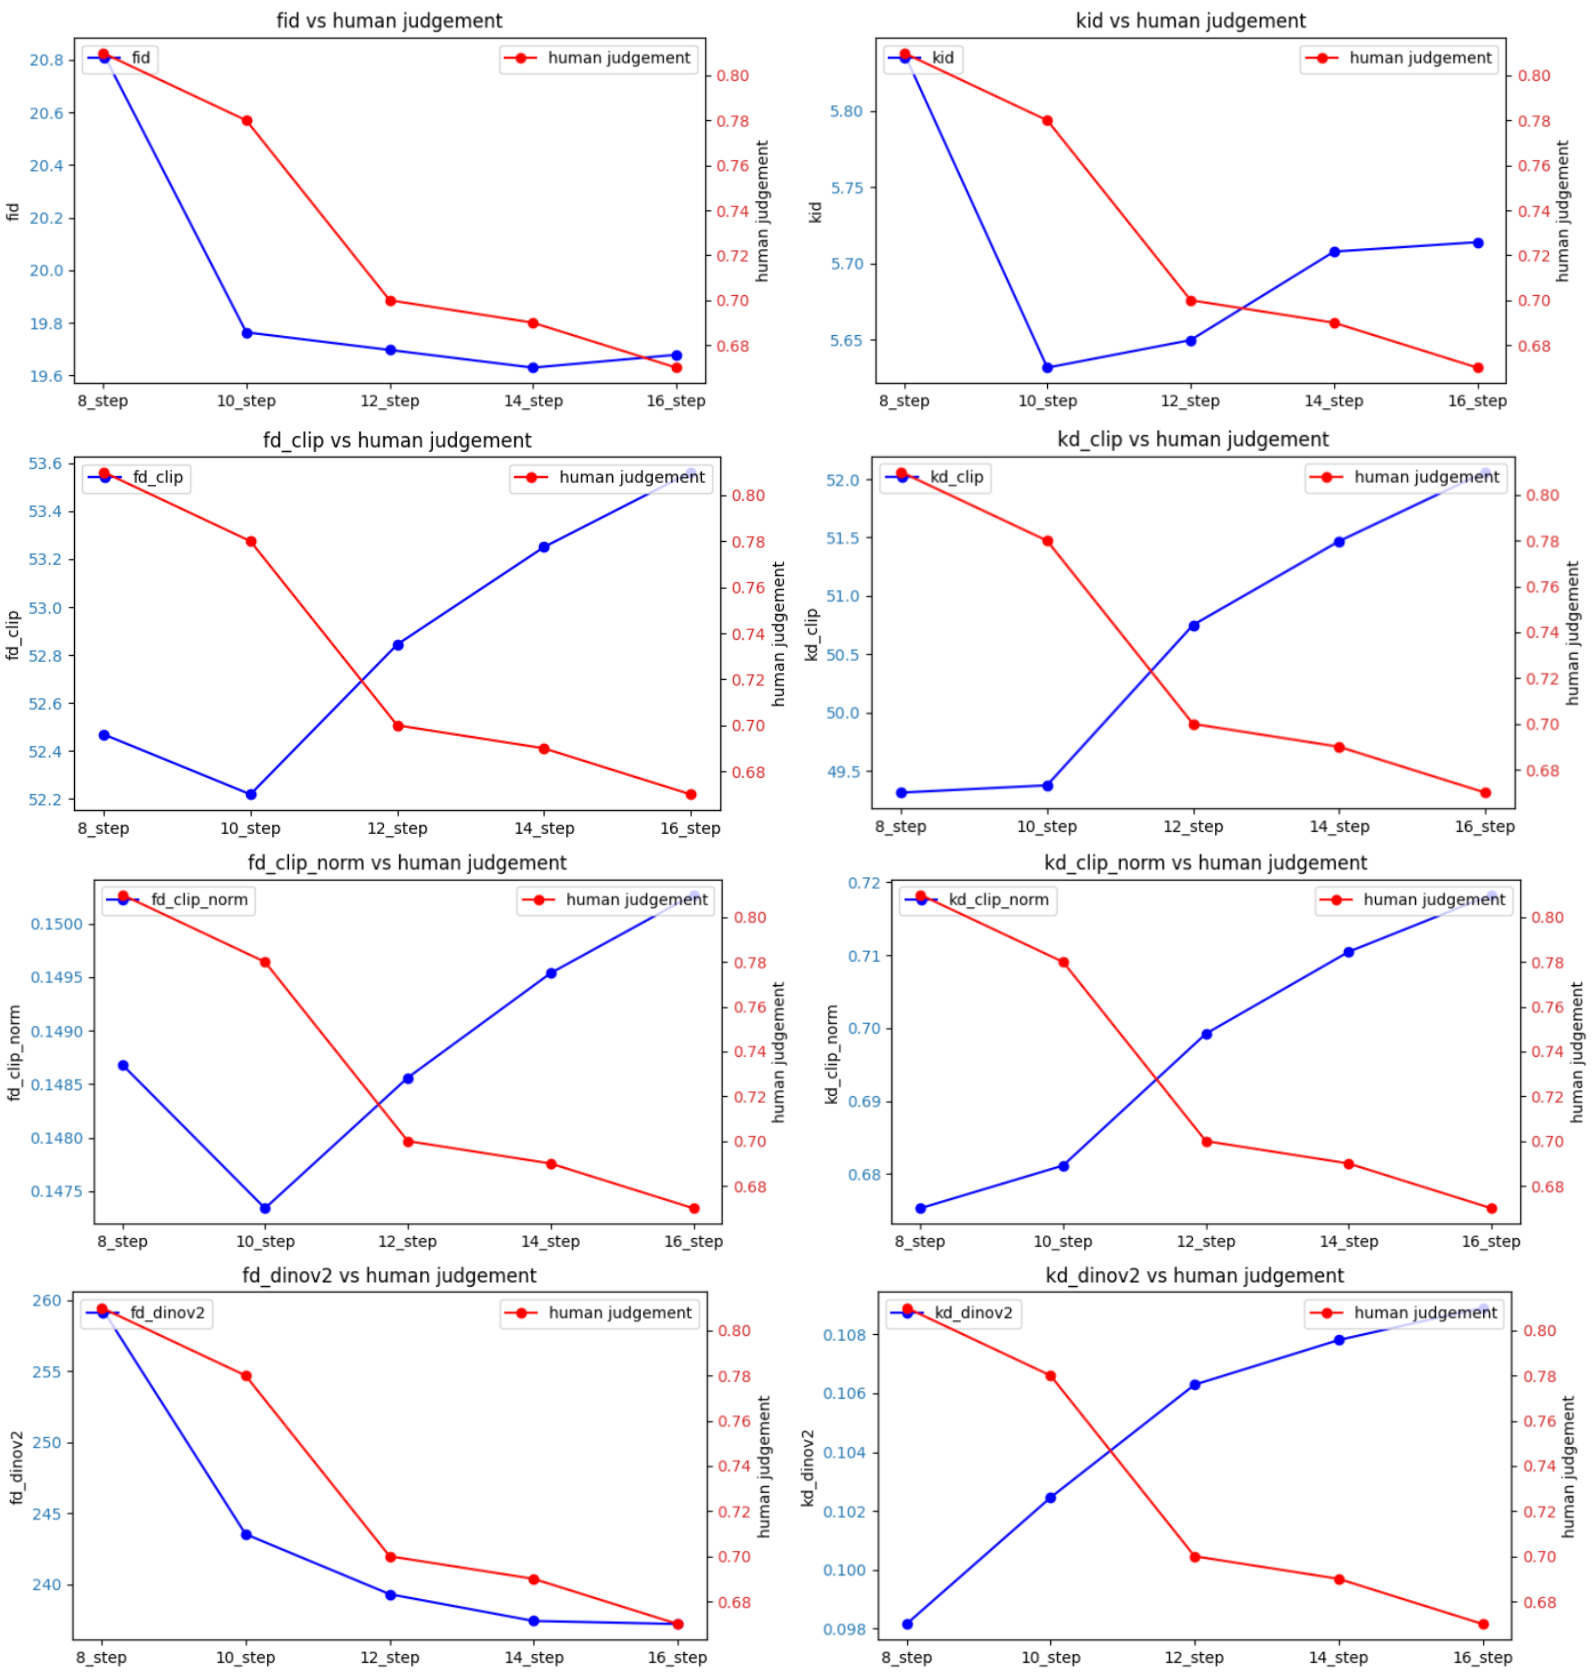
\includegraphics[width=16cm, height=17cm]{figs/coco_gen_steps.png}
\caption{Distance metrics measured on COCO dataset on models with different number of de-noising(generation) steps. On the X-axis from left to right there are models with different number of steps from smaller to larger, i.e. from 8 steps to 16 steps. The left Y-axis shows the results of the metric, so the blue graph corresponds to the left Y-axis. On the right side of the Y-axis are the human evaluation results, which is the proportion of wins in the 16-step model against the current model with the current number of de-noising steps. The red graph corresponds to the right Y-axis.}
\label{fig:coco_gen_steps}
\end{figure}

\begin{figure}[]
\centering
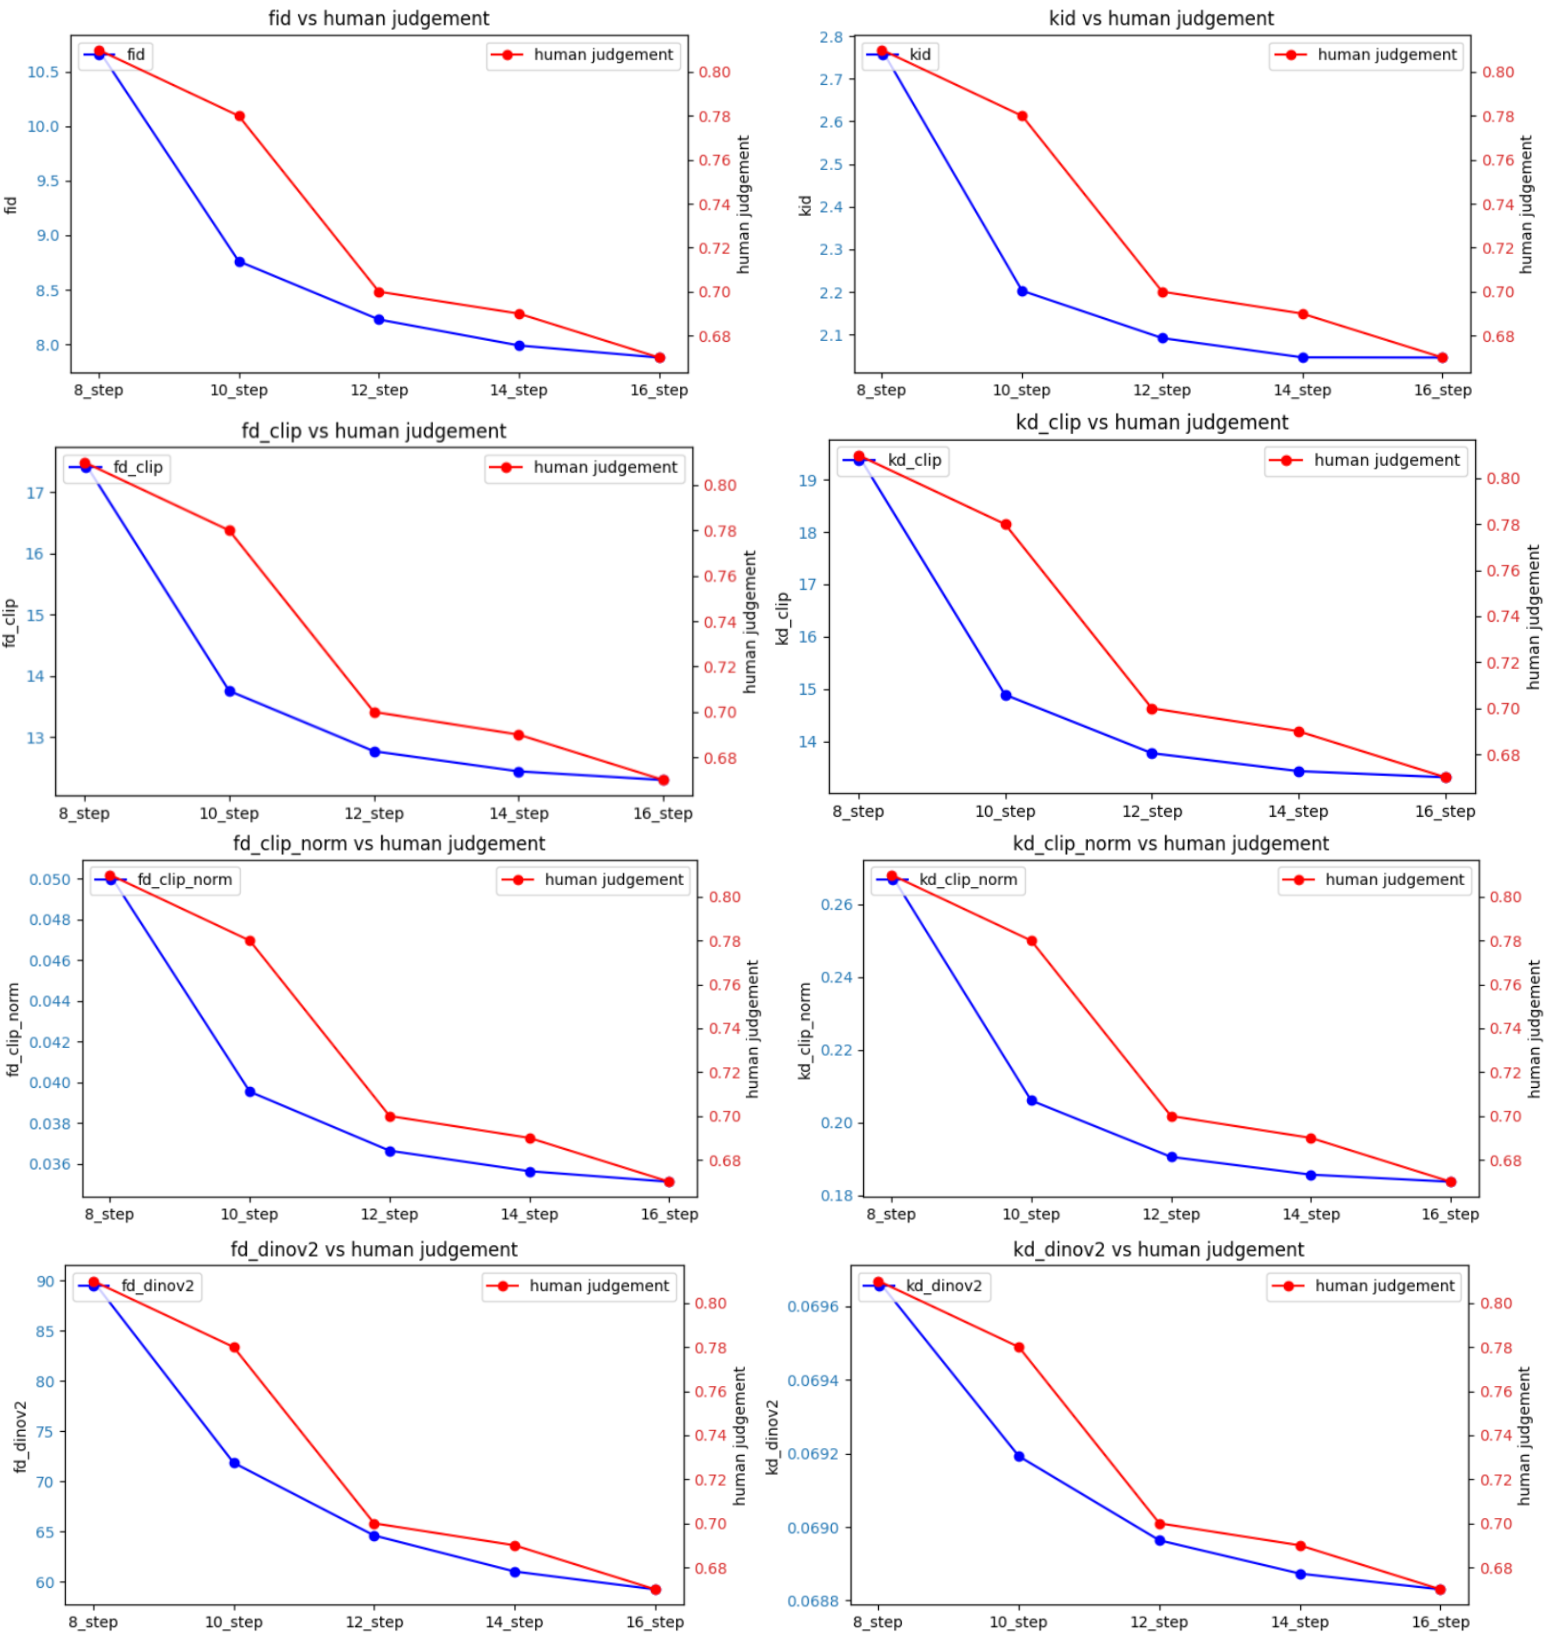
\includegraphics[width=16cm, height=17cm]{figs/mjhq30k_gen_steps.png}
\caption{Distance metrics measured on MJHQ30K dataset on models with different number of de-noising(generation) steps. The axes are the same on the Figure\ref{fig:coco_gen_steps}.}
\label{fig:mjhq30k_gen_steps}
\end{figure}

\subsubsection{Summary}
At the end of this experiment I can say that the FD\_DINOv2 metric performed the best. FID also showed excellent results. KID, FD\_CLIP, KD\_CLIP, FD\_CLIP\_norm and KD\_CLIP\_norm show poor results which may doubt CLIP as feature extractor. KD\_DINOv2 showed excellent results on the MJHQ30k dataset, but the exact opposite on COCO.

In this experiment, my assumption that KD\_DINOv2 shows correlation between generated images and MJHQ30k dataset and does not show with COCO because the model generates more contrasty and aesthetic images was confirmed.

After two experiments, I decided to remove metrics from CLIP as feature extractor since they show the worst results.

\subsection{Corrupted images by overlaying black squares on the images}
The third experiment I did was to corrupt the images that the model generated. I added black squares to the generated images and intuitively expected that the metric should show that the performance of the model was degraded. The idea for the experiment was taken from the original FID metric paper\cite{FID}.


It is important to note that I added black squares exactly on the generation items in the image. For example, if the prompt was “squirrel sitting on a tree”, then I put the square exactly on the part of the squirrel, not on the background of the image. At the Figure \ref{fig:images_with_black_squares} I show images generated images with black squares.

\begin{figure}[]
\centering
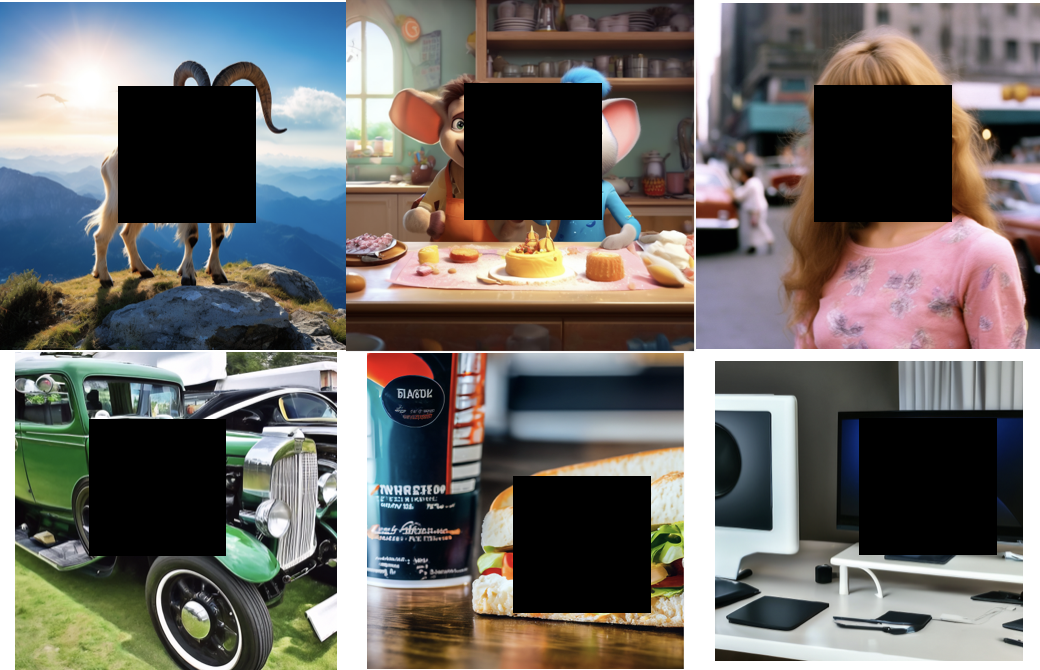
\includegraphics[width=7cm, height=6cm]{figs/images_with_black_squares.png}
\caption{Generated images with black squares.}
\label{fig:images_with_black_squares}
\end{figure}

\subsubsection{Summary}
As a result of the experiment, all metrics showed that pictures with painted black squares are worse, that is, less similar to the pictures from the dataset. Therefore, no additional information can be extracted from the experiment, because all metrics have performed perfectly.

\subsection{COS\_DINOv2 metric}
Separately, I conducted experiments for the COS\_DINOv2 metric, which I described in the “Methodology” chapter. I conducted two experiments: different numbers of de-noising steps and training steps. I used two datasets: COCO and MJHQ30k.

In all four experiments, the metric performed admirably. It correlates with human judgment in all experiments.

\begin{figure}[]
\centering
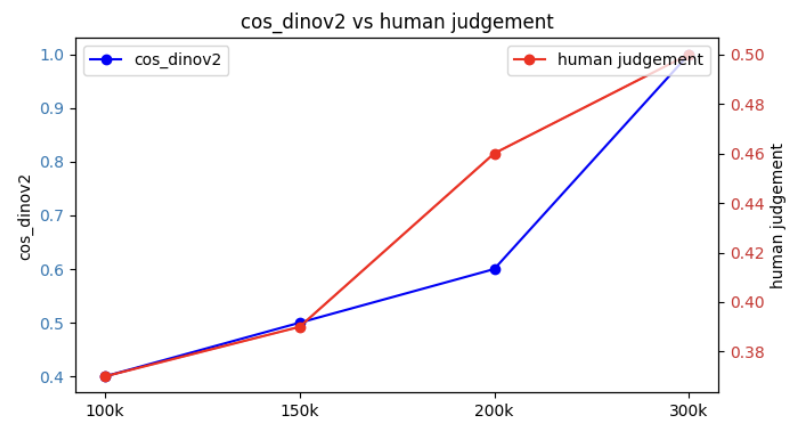
\includegraphics[width=9cm, height=5cm]{figs/coco_train_steps_COS_DINOv2.png}
\caption{COS\_DINOv2 on COCO dataset with different number of train steps. On the X-axis from left to right there are models with different number of steps from smaller to larger, i.e. from 100 thousand to 300 thousand. The left Y-axis shows the results of the metric, so the blue graph corresponds to the left Y-axis. On the right Y-axis are the results of human evaluation - this is the proportion of victories of the current model with the current number of training steps against the fully trained model (i.e. the model with 300 training steps). The red graph corresponds to the right Y-axis.}
\label{fig:coco_train_steps_cos_dinov2}
\end{figure}

\begin{figure}[]
\centering
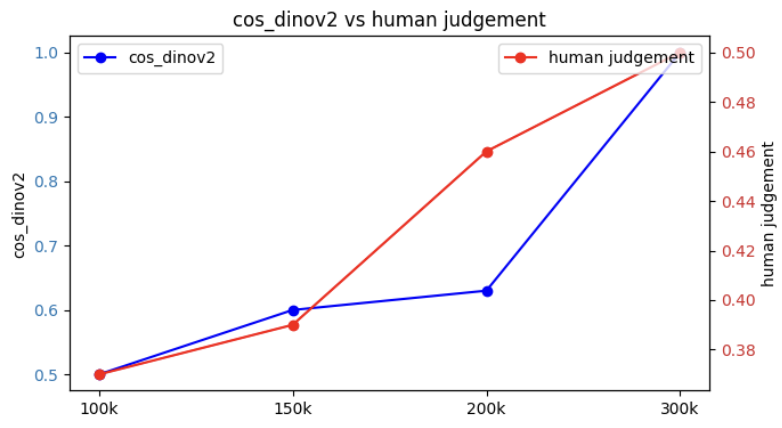
\includegraphics[width=9cm, height=5cm]{figs/mjhq30k_train_steps_COS_DINOv2.png}
\caption{COS\_DINOv2 on MJHQ30k dataset with different number of train steps. The axes are the same on the Figure \ref{fig:coco_train_steps_cos_dinov2}.}
\label{fig:mjhq30k_train_steps_cos_dinov2}
\end{figure}

\begin{figure}[]
\centering
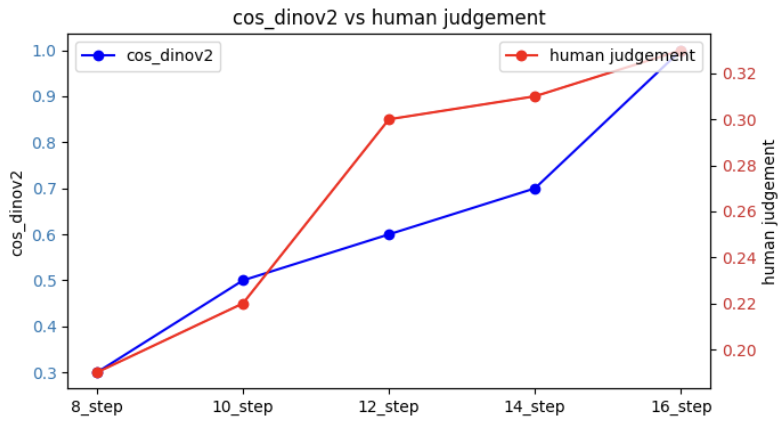
\includegraphics[width=9cm, height=5cm]{figs/coco_gen_steps_COS_DINOv2.png}
\caption{COS\_DINOv2 on COCO dataset with different number of de-noising steps. On the X-axis from left to right there are models with different number of steps from smaller to larger, i.e. from 8 steps to 16 steps. The left Y-axis shows the results of the metric, so the blue graph corresponds to the left Y-axis. On the right side of the Y-axis are the human evaluation results, which is the proportion of wins in the current model with the current number of de-noising steps against the 16-step model. The red graph corresponds to the right Y-axis.}
\label{fig:coco_gen_steps_cos_dinov2}
\end{figure}

\begin{figure}[]
\centering
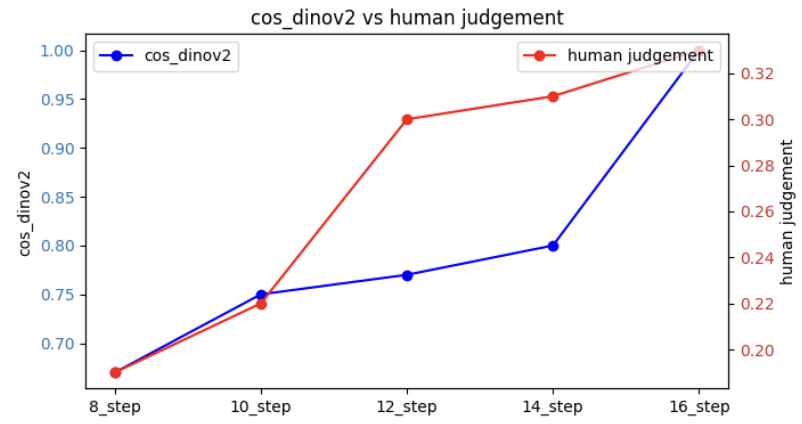
\includegraphics[width=9cm, height=5cm]{figs/mjhq30k_gen_steps_COS_DINOv2.png}
\caption{COS\_DINOv2 on MJHQ30k dataset with different number of de-noising steps. The axes are the same on the Figure \ref{fig:coco_gen_steps_cos_dinov2}.}
\label{fig:mjhq30k_gen_steps_cos_dinov2}
\end{figure}

\subsection{Summary for experiments with distance metrics}
From all the experiments performed, two metrics can be highlighted: FD\_DINOv2 and COS\_DINOv2. These are the metrics that show a precise correlation with human opinion in all experiments.

\section{Experiments with score metrics}
With scoring metrics, I did one experiment. It was to train Imagen with different number of steps and see how the metrics would behave. I use four metrics in total: CLIPScore\cite{CLIPScore}, CLIPSCore with MCLIP, ImageReward\cite{Image_reward}, HPSv2\cite{HPSv2} .I use the same models I used in the distance metrics experiments. I used the prompts from the COCO dataset. The resulting graphs of the experiment are shown in Figure \ref{fig:coco_train_steps_score_metrics}.

\begin{figure}[]
\centering
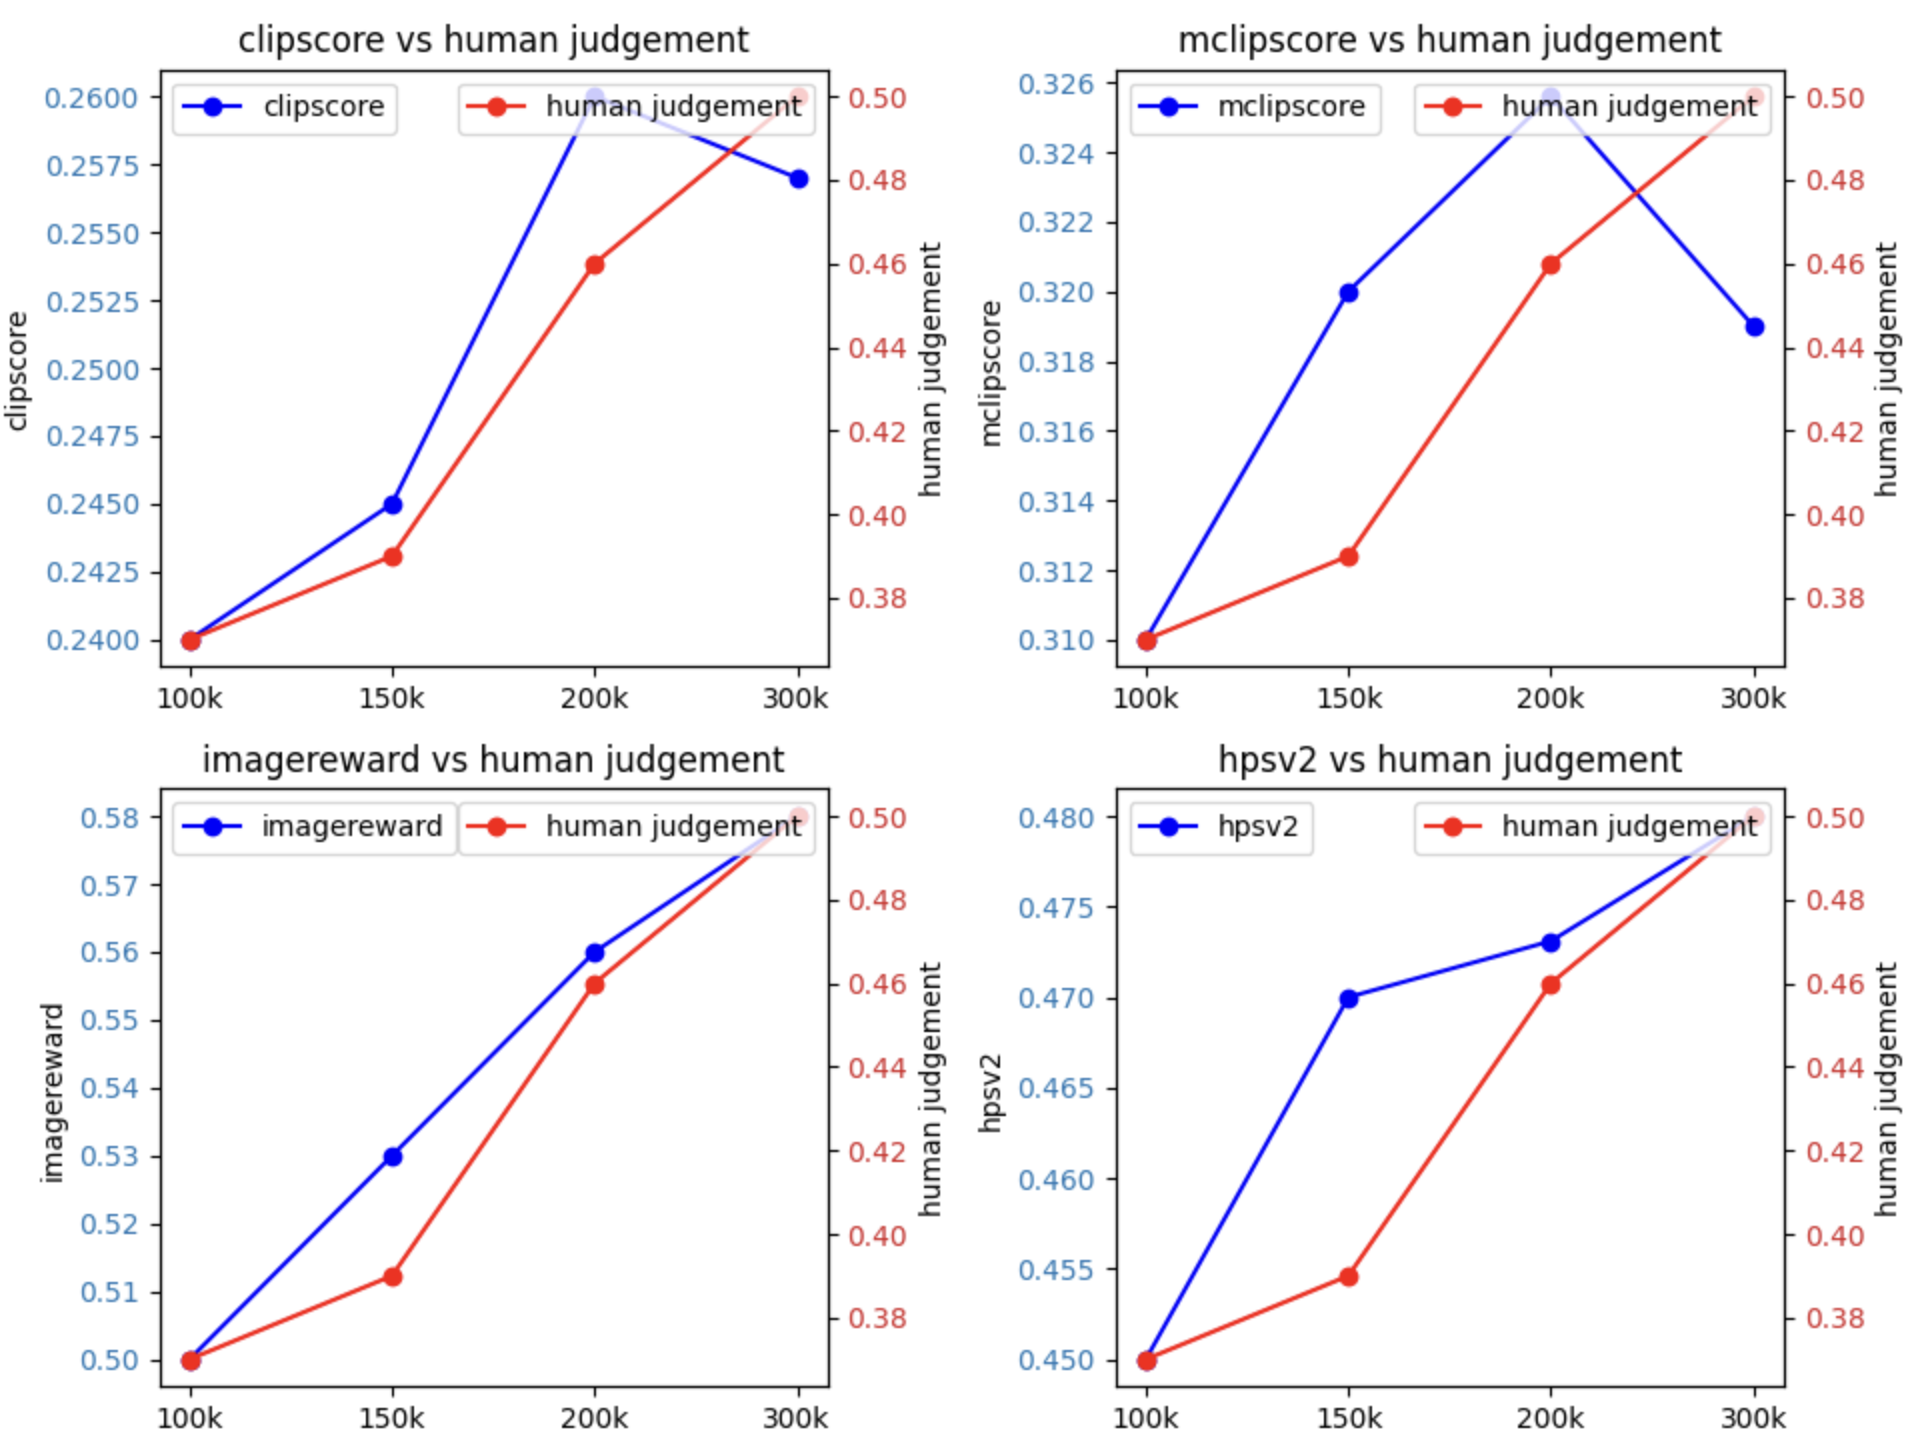
\includegraphics[width=15cm, height=9cm]{figs/coco_train_steps_score_metrics.png}
\caption{Score metrics on COCO dataset with different number of train steps. The axes are the same on the Figure \ref{fig:coco_train_steps_cos_dinov2}.}
\label{fig:coco_train_steps_score_metrics}
\end{figure}

My experiment shows similarity of CLIPScore and CLIPScore metrics on MCLIP feature extractor, also it can be seen that ImageReward and HPSv2 correlate better with human judgement than CLIPScore and CLIPScore on MCLIP chips. ImageReward correlates best of all so it becomes the leader in score metrics.
